\section{Boomerang Design}

As previously discussed, the Boomerang protocol enhancement for Bitcoin is motivated by the need to hide the source from which transactions are introduced into the network. Furthermore, this should be done in a transparent way so that any other form of anonymous coin extension on top of Bitcoin (e.g., Zerocoin) can leverage the service for transaction anonymity. Boomerang is \emph{not} intended to support regular Bitcoin traffic; once a transaction becomes public knowledge, Boomerang no longer plays a role in its distribution. 

In the following sections we detail the core protocol and several important design and security tradeoffs that can be made in practice when using Boomerang. A formal analysis of the security and performance of Boomerang-enhanced Bitcoin is provided in Sections X and Y. 

\subsection{Broadcast Protocol}

At the heart of the Bitcoin protocol is the ability to encode new transactions as Boomerang messages and then ripple them throughout the network. We describe the complete procedure for message encoding, {\sf EncodeTransaction}, in Algorithm \ref{alg:encode}, where the notation contained therein is defined in Table \ref{tab:notation}. An encoded Boomerang message has a very well-defined format, as shown in Figure \ref{fig:boomerang_message}. In particular, the message is composed of the following:
\begin{enumerate}
	\item A potentially re-encrypted seed. By the description of {\sf EncodeTransaction}, it is required that the public-key encryption scheme used to mask these seeds has the same domain and range. This is needed because the decrypted seed for one hop will be used as decrypted seed on the previous hop, very much like onion layers of encryption.
	\item An encrypted address vector that is used by each hop to learn the next hop in the circuit without learning any other information about the nodes in the circuit. More specifically, a router can only learn about the immediate source and destination of a Boomerang message (the security and anonymity implications of this are discussed in the following section).
	\item A potentially re-encrypted transaction message block. This block either stores the encrypted transcaction, where the encryption is done by XORing with a pseudorandom bit string generated by the decrypted seed value, or the plaintext transaction that is to be broadcast throughout the network.
\end{enumerate}

\begin{table*}[ht!]
\begin{center}
\caption{Boomerang Protocol Notation}
	\begin{tabular}{|l|l|}\hline
	\textbf{Symbol} & \textbf{Description} \\ \hline
	~ & ~ \\
	~ & ~ \\
	~ & ~ \\ \hline
	\end{tabular}
\end{center}
\end{table*}

\begin{figure}[ht!]
\begin{center}
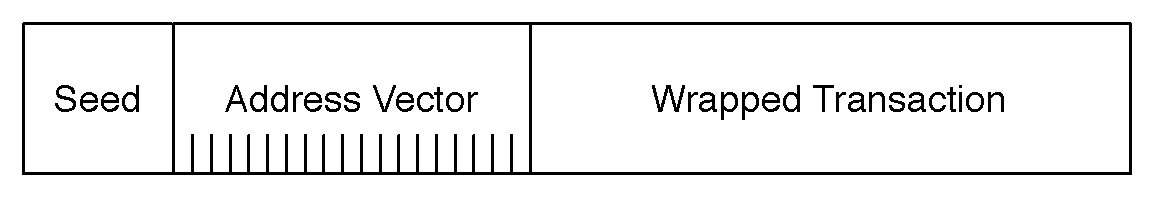
\includegraphics[scale=0.4]{./images/boomerang_message.pdf}
\caption{Boomerang message encoding.}
\label{fig:boomerang_message}
\end{center}
\end{figure}

The procedure to handle Boomerang messages, {\sf BoomerangMessageHandler}, is provided in Algorithm \ref{alg:handler}. 

\begin{algorithm*}[t!]
\caption{{\sf EncodeTransaction}($T$)}
\label{alg:encode}
\begin{algorithmic}[1]

\For{$m = 1$ to $M$}
	\State $\bar{T} := T$
	\State $s \gets \{0,1\}^{\tau}$
	\For{$n = 1$ \textbf{to} $N_m$}
		\State $p := \mathsf{PRG}(s)$
		\State $\bar{T} := \bar{T} \oplus p$
		\State $s \gets E_{pk_{m,n}}(s)$
	\EndFor

	% populate the address vector
	\State $\mathsf{index} \gets \{0,\dots,2N_m\}$ % random address vector index
	\State $\mathsf{AV} := [2N_m]$ % address vector
	\For{$n = N_m$ \textbf{downto} $2$}
		\State $\mathsf{AV}[\mathsf{index}] := E_{pk_{m,n}}(\mathsf{addr}_{N_n})$
		\State $\mathsf{index} := \mathsf{index} + 1 (\mod N_m)$
		\State $\mathsf{AV}[\mathsf{index}] := E_{pk_{m,n}}(\mathsf{addr}_{N_{n-1}})$
		\State $\mathsf{index} := \gets \{0,\dots,2N_m\}$
		\While {$\mathsf{index} \mod 2 \not= 0$ \text{ and } $\mathsf{AV}[\mathsf{index}] \not= \bot \text{ and } \mathsf{AV}[\mathsf{index + 1 (\mod N_m)}] \not= \bot$}
			\State $\mathsf{index} \gets \{0,\dots,2N_m\}$
		\EndWhile
	\EndFor

	\State $M := \mathsf{Pack}(s, \mathsf{AV}, \bar{T})$
	\State $\mathsf{Transmit}(M)$
\EndFor

\end{algorithmic}
\end{algorithm*}

\begin{algorithm*}[t!]
\caption{{\sf BoomerangMessageHandler}($n$, $M$)}
\label{alg:handler}
\begin{algorithmic}[1]

\State $s := D_{sk_{n}}(M[0])$
\State $\bar{T} := M[2] \oplus PRG(s)$
\If {$\bar{T}$ is a well formed transaction}
	\State $\mathsf{Broadcast}(\bar{T})$ to the Bitcoin network
\ElsIf {$\bar{T}$ destination address is $\mathsf{addr}_n$}
	\State Discard $\bar{T}$; return;
\Else
	\State $\mathsf{AV} := M[1]$
	\State $n := 1$
	\While {$n < 2N_m$}
		\State $\mathsf{addr}_{src} := D_{pk_n}(AV[n])$
		\If {$\mathsf{addr}_{src} = \mathsf{addr}_n$}
			\State $\mathsf{addr}_{dst} := D_{pk_n}(AV[n + 1])$
			\State $M := \mathsf{Pack}(s, \mathsf{AV}, \bar{T})$
			\If {$|Buffer| \geq B$}
				\State $\mathsf{Transmit}(M)$
			\Else
				\State $B.add(M)$
			\EndIf
		\Else
			\State $n := n + 2$
		\EndIf
	\EndWhile
\EndIf

\end{algorithmic}
\end{algorithm*}

% TODO: cover traffic generation, mix delay

Similar to the Tarzan P2P mixnet, a critical part of the Boomerang protocol is the inclusion of cover traffic that is indistinguishable from legitimate encoded Boomerang transaction messages \cite{tarzan}. This traffic is needed for two reasons: (1) to keep legitimate transactions moving through mixnet circuits, and (2) to obfuscate the flow of legitimate transactions through the network. To support this cover traffic with minimal changes to the protocol, nodes in the network will \emph{reuse} and \emph{re-encode} old transactions to be sent throughout the network, with the exception that the destination node for the mixnet circuit (as specified in the {\sf EncodeTransaction} procedure) will be the same as the sender. This is because the sender can easily discover when a transaction message has looped through the network and back to themselves, at which point they can then simply discard the transaction. Clearly, the rate at which this cover traffic is generated plays a critical role in the overall performance of the system when using Boomerang. We discuss the selection of parameters that achieve optimal performance without sacrificing security in Section 5. 

\subsection{Cryptographic Primitives}

% TODO: PRG, PK-encryption, etc

Based on the {\sf EncodeTransaction} and {\sf BoomerangMessageHandler} procedures, we require the following cryptographic primitives to support Boomerang messages:
\begin{enumerate}
	\item Uniform domain and range public-key encryption without ciphertext expansion, and
	\item Deterministic PRG whose input is an element in the range specified by the public-key encryption scheme.
\end{enumerate}

% TODO: rsa & prg

% \begin{figure}[ht!]
% \begin{center}
% 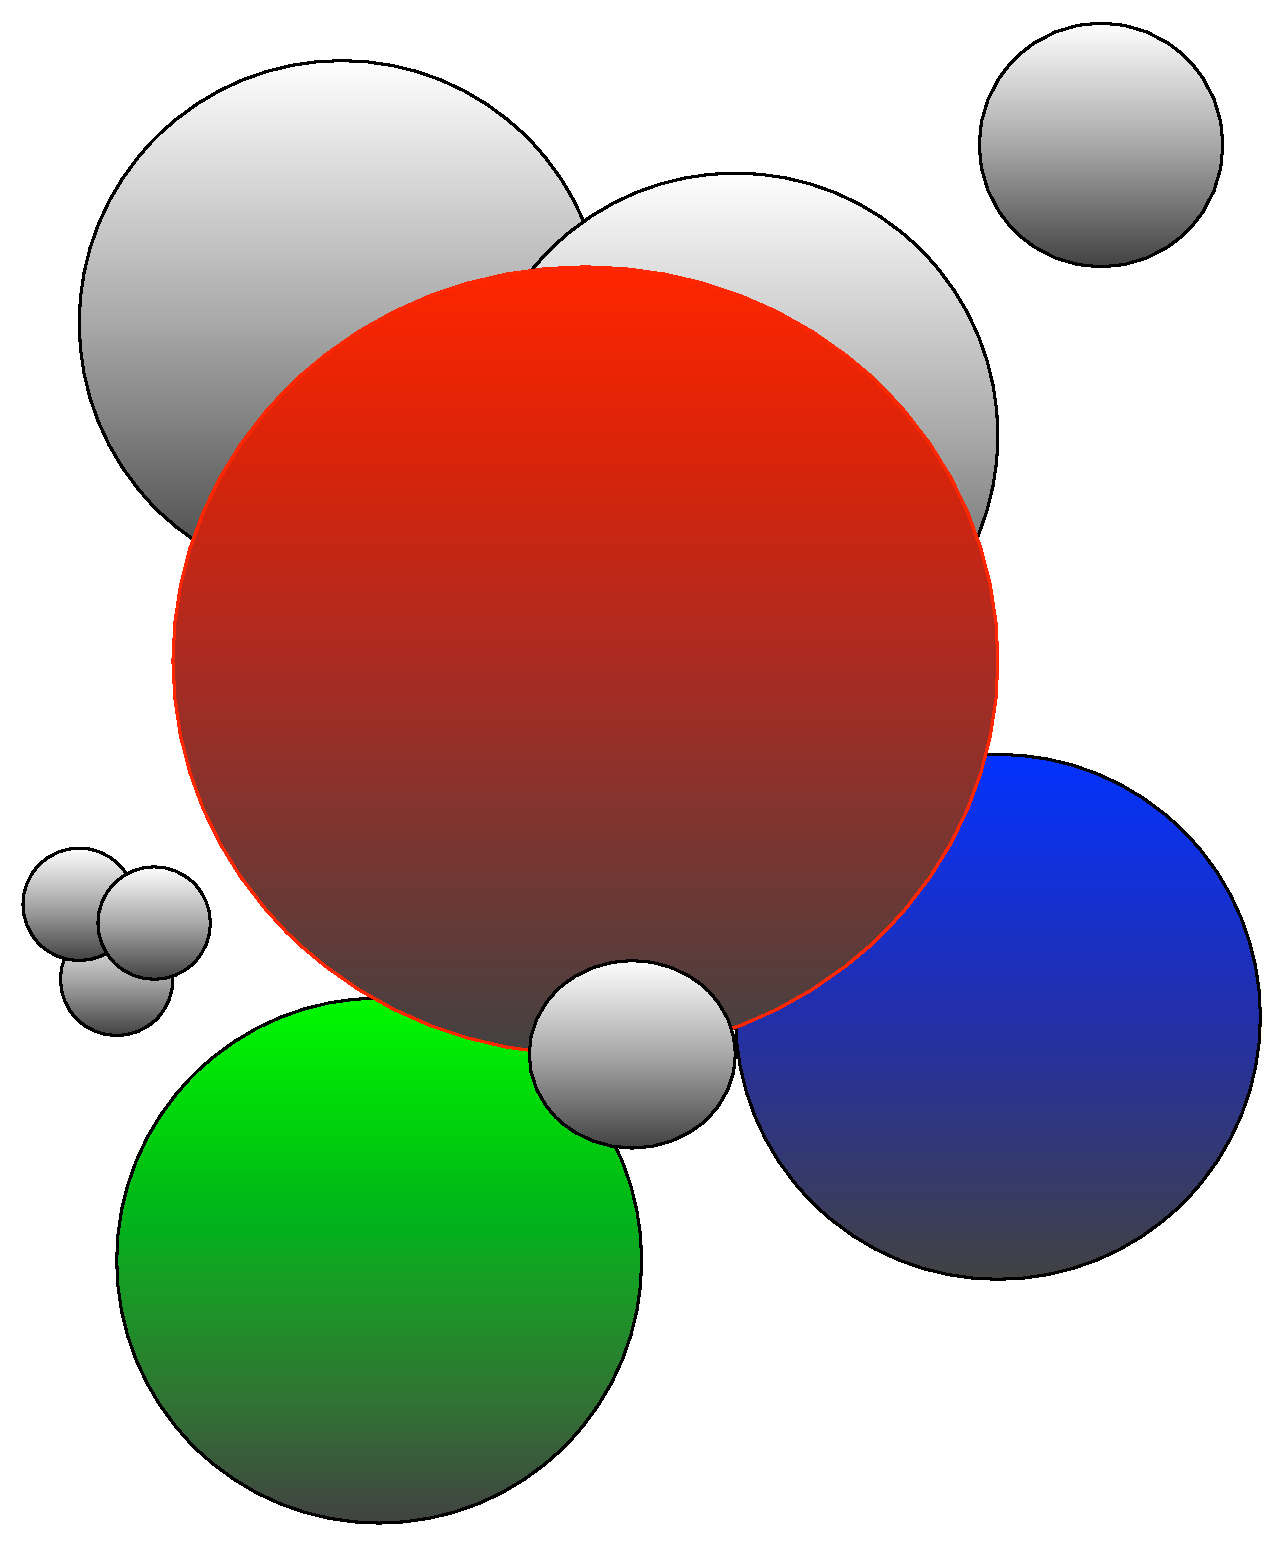
\includegraphics[scale=0.25]{./images/boomerang_clusters.pdf}
% \caption{TODO}
% \label{fig:boomerang_clusters}
% \end{center}
% \end{figure}

